\subsection{第 14 课 | 高级搜索}

\subsubsection{脑图}

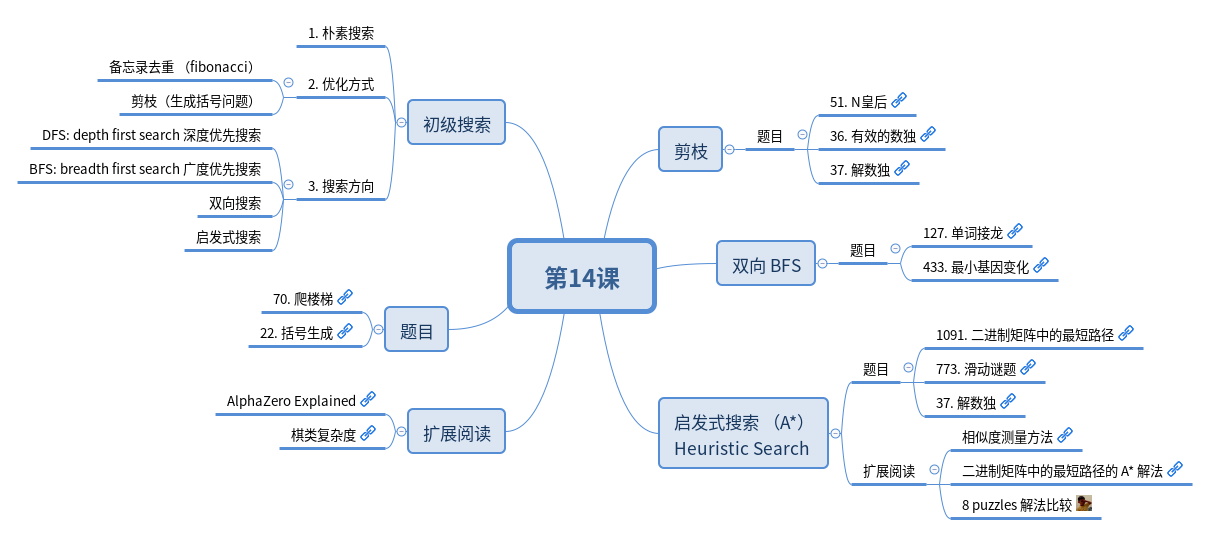
\includegraphics[width=140mm,height=60mm]{images/camp/第14课.png}

\subsubsection{题目}

\begin{itemize}
  \item \hyperref[leetcode:70]{70. 爬楼梯}
  \item \hyperref[leetcode:22]{22. 括号生成}
  \item \hyperref[leetcode:51]{51. N皇后}
  \item \hyperref[leetcode:36]{36. 有效的数独}
  \item \hyperref[leetcode:37]{37. 解数独}
  \item \hyperref[leetcode:127]{127. 单词接龙}
  \item \hyperref[leetcode:433]{433. 最小基因变化}
  \item \hyperref[leetcode:1091]{1091. 二进制矩阵中的最短路径}
  \item \hyperref[leetcode:773]{773. 滑动谜题}
\end{itemize}
